
\section{Lo sviluppo di una memoria locale}

Richiedere e ottenere dati dal server comporta ritardi che impattano sulle prestazioni. 
Se la tecnologia del dispositivo lo permette, è utile salvare copie delle informazioni usate più frequentemente nella memoria locale del dispositivo. 
Nel momento di una interazione che richiede la ricerca dei dati, si possono fornire le informazioni disponibili in copia, 
per poi eventualmente aggiornarle se si rivelassero imprecise. Questo permette un tempo di risposta apparente minore e una migliore esperienza utente.\\
\\

\subsection{L'implementazione della cache}
Non tutti i dispositivi permettono una gestione della memoria a lungo termine. 
In particolare, i browser web non presentano questa funzionalità, ma i dispositivi mobili e i programmi sì. \\
\\
Per motivi di prestazioni, il framework Flutter nativamente mantiene lo stato di un componente solo il tempo strettamente necessario per la sua esecuzione. 
Il tempo di vita dello stato coincide normalmente con quello del componente a cui è associato. 
La normale persistenza degli elementi e dei dati ha durata limitata. 
Si rende necessaria la creazione e la gestione di una cache locale che permetta di mantenere i dati ricevuti dal server anche in seguito al termine di servizio dei componenti.\\
\\
\begin{figure}[h!]
    \centering
    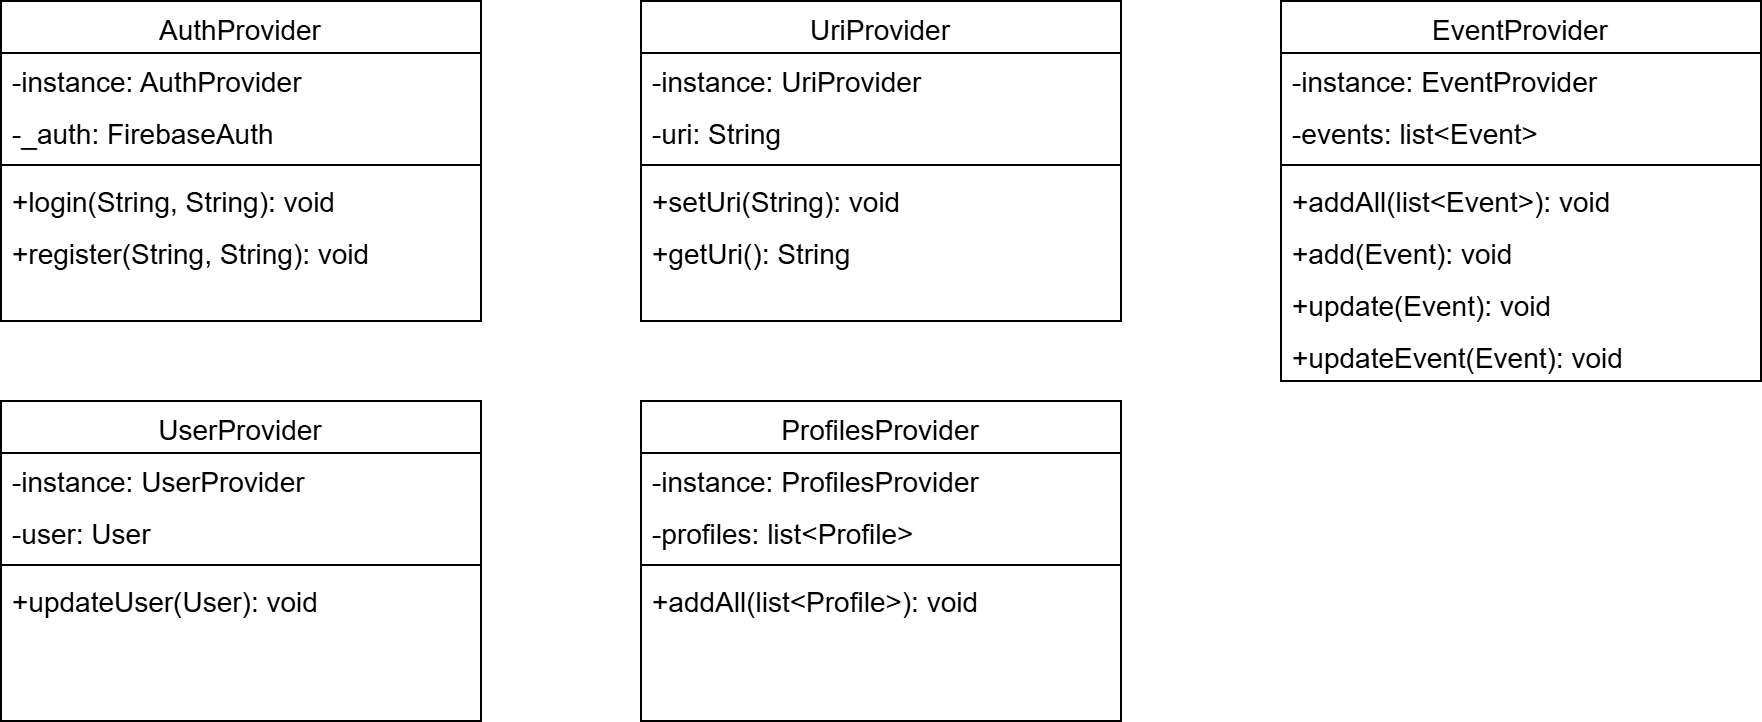
\includegraphics[width=\textwidth]{FrontProviderClassDiagram.png}
    \caption{Classi provider all'interno dell'applicazione}
\end{figure}	
La cache locale viene suddivisa in base alle classi logiche del dominio, ed è accessibile tramite servizi dedicati. 
In particolare, grazie a componenti di tipologia provider è possibile aggiornare in automatico le parti dell’applicazione interessate dalle modifiche. 
Al termine di una richiesta dati al server, il provider viene notificato, salvando il dato in memoria e scatenando un aggiornamento a catena sui componenti interessati.\\
\\
La cache deve essere unica e disponibile in tutto il programma. 
I provider attraverso cui si realizza la cache locale seguiranno il pattern singleton, che garantisce l’unicità dell’elemento all’interno del programma. 
Una volta creati all’avvio del programma, infatti, tutti gli elementi dell’applicazione avranno accesso agli stessi dati, quando necessario.

\begin{figure}[h!]
    \centering
    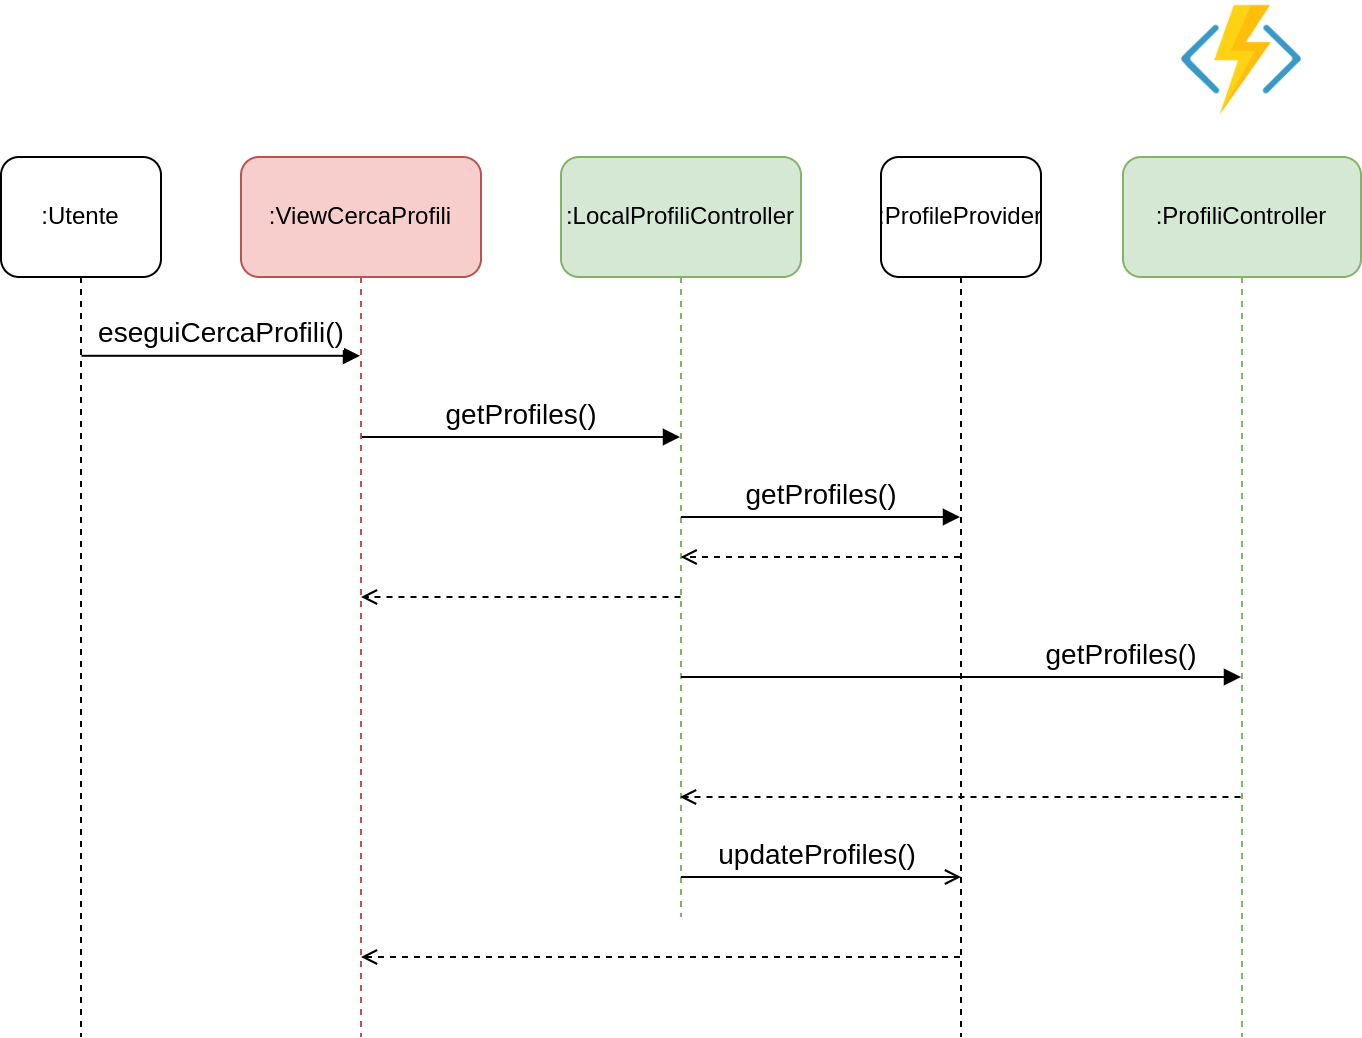
\includegraphics[width=\textwidth]{Providers.png}
    \caption{Esempio di interazione logica tra i componenti del client}
\end{figure}	
\clearpage

\subsection{L'allineamento con la memoria centrale}

il client ha la responsabilità di tenere allineata la propria cache ai valori della memoria centrale. 
Per quanto possa fare temporaneamente affidamento sulle risorse che ha salvato in cache per ridurre i tempi di risposta con l’utente, 
la loro validità dipende dalla certezza che corrispondano ai dati ufficiali. \\
\\

Ogni elemento avrà associato l’ultimo momento in cui è stato aggiornato. 
Allo stesso modo, viene salvato l’ultimo momento in cui è stata attivamente effettuata una richiesta esplicita di aggiornamento.  
Ad ogni avvio dell’applicazione il client invierà una richiesta al server per ricevere tutti gli elementi che hanno subito modifiche successivamente al momento dell’ultimo aggiornamento.\\
\\
La necessità di avere aggiornati tutti gli elementi della cache nel minor tempo possibile dipende anche dalla tipologia dell’elemento. 
Bisogna identificare gli elementi per il quale l’allineamento è critico per il corretto funzionamento dell’applicazione, 
come invece quelli che svolgono ruoli secondari e possono essere aggiornati anche in un secondo momento. 
Ad esempio, la modifica della durata di un evento è necessario venga rilevata il prima possibile, 
mentre la modifica della foto associata ad un profilo ha vincoli di aggiornamento in memoria locale molto più rilassati.\\
\\
Nel caso di dati critici si implementa un meccanismo che esegue, periodicamente, una richiesta degli elementi modificati nell’arco di tempo dall’ultimo aggiornamento, 
per poi aggiornare il loro valore. Invece, nel caso di elementi secondari, 
si possono richiedere allineamenti direttamente nel momento in cui vengono posti espressamente in attenzione dato l’utilizzo dell’app.

\clearpage
\section{La sincronizzazione tra la cache locale e la memoria principale}

Data la natura condivisa dell’applicazione risulta fondamentale che gli utenti siano aggiornati in tempo reale sulle modifiche applicate agli eventi, 
oltre ad essere una prerogativa di tutte le applicazioni moderne, anche per migliorare la user experience. 
Lo spostamento di un appuntamento, la conferma di una presenza o la modifica del luogo di appuntamento sono elementi critici che è bene che gli utenti vengano informati il prima possibile. \\
\\
Il cloud fornisce strumenti per il supporto e lo sviluppo di queste funzionalità, ma, oltre a dover individuare la tecnologia più adatta, bisogna anche essere in grado di integrarla nel resto del progetto.\\
\\
\subsection{La scelta della tecnologia}


La comunicazione con il server finora implementata si basa sul protocollo Hypertext Transfer Protocol (HTTP). HTTP prevede un fornitore di servizi (il server) mettere a disposizione una porta ad un indirizzo fisso rimanendo in attesa di eventuali utilizzatori (client) che, interfacciandosi attivamente alla porta disponibile,  espongono le loro richieste.
La riduzione delle comunicazioni al minimo indispensabile, oltre a non richiedere al server alcuna conoscenza del client, rende il protocollo pratico e scalabile.

Questa dinamica però impedisce ai client di essere notificati di eventuali modifiche apportate, a meno di richieste periodiche frequenti che comportano un sovraccarico da entrambe le parti. Inoltre, l’inversione dei ruoli non è applicabile in quanto i client cambiano costantemente l’indirizzo a loro associato, così come è impossibile distinguere se il dispositivo abbia terminato la connessione o se sia un guasto di altro tipo. 

Si necessita una comunicazione che mantenga in costante contatto i client con le modifiche del server, permettendo una trasmissione attiva degli aggiornamenti.
A basso livello, il protocollo che permette una comunicazione continua più adatto alle tecnologie comunemente diffuse è quello delle WebSocket. Tramite WebSocket infatti si crea un canale diretto tra le parti che consente una comunicazione istantanea. 

Alla necessità di supportare il protocollo delle WebSocket e di inviare istantaneamente i messaggi, si aggiunge la possibilità di creare molteplici canali specifici per indirizzare correttamente le comunicazioni ai soli interessati.


\begin{figure}[h!]
    \centering
    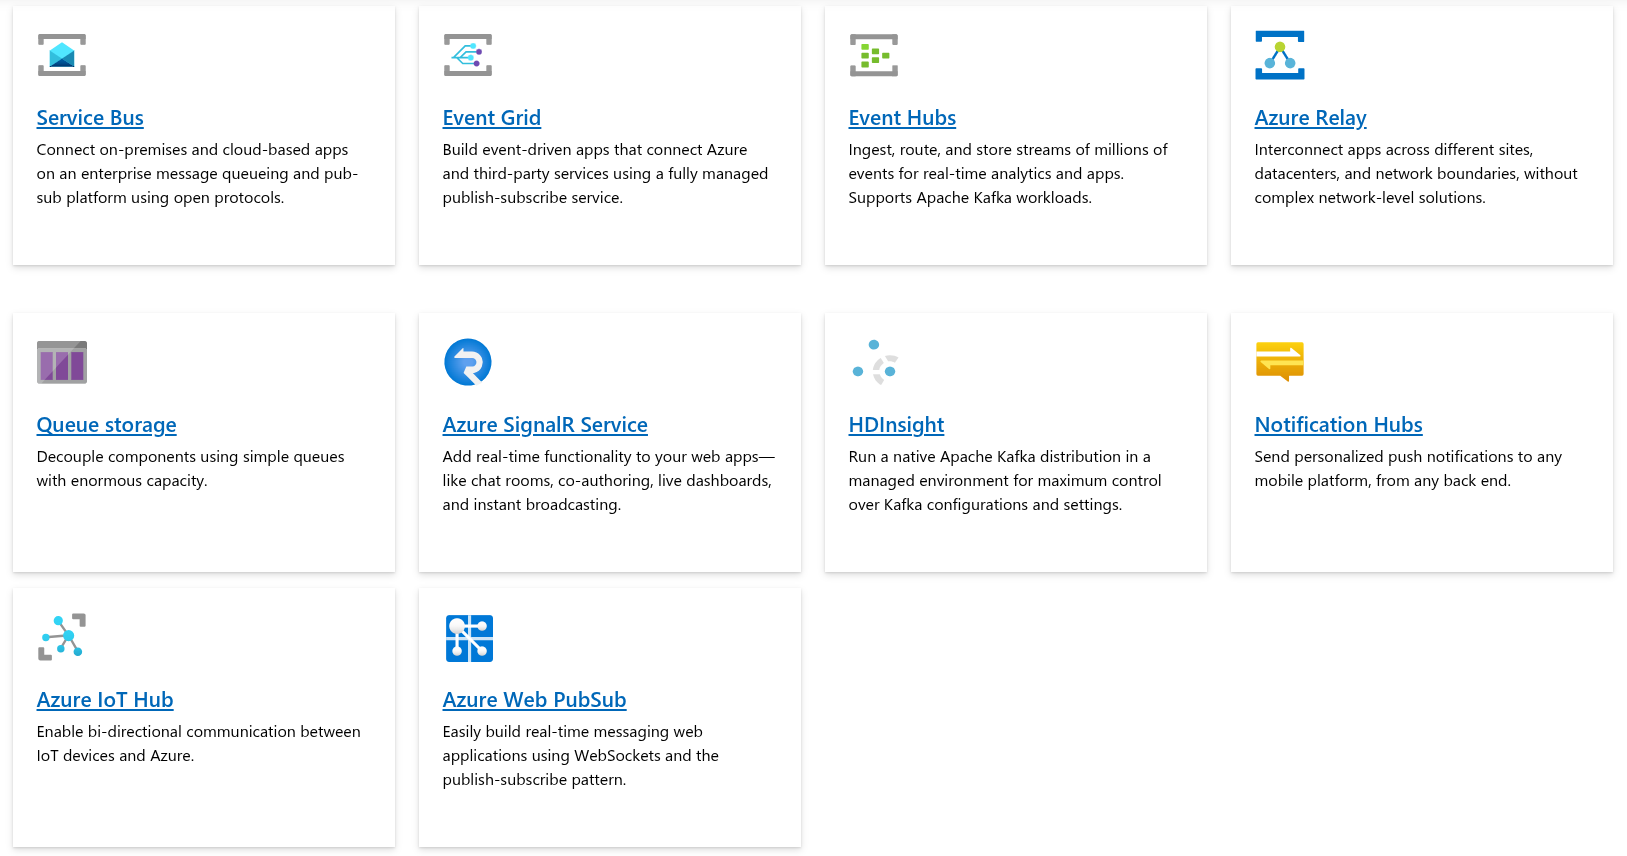
\includegraphics[width=\textwidth]{AzureMessagingServices.png}
    \caption{I servizi di comunicazione istantanea proprietari di Azure}
\end{figure}	


Per individuare la tecnologia più adatta ad aggiornare gli utenti, tra le tante che offrono servizi di collegamento istantaneo tra tecnologie, è fondamentale comprendere  gli scopi per cui sono nate e che problemi quindi risolvono. Infatti, ogni servizio è stato progettato per affrontare specifiche sfide che si differenziano sia per la natura dei servizi a cui si rivolgono che per  modalità di approccio .

La natura degli attori per cui il servizio si specializza determina le prestazioni di scalabilità e le integrazioni supportate. Bisogna quindi considerare la località e la natura delle risorse: in-premise o sul cloud, se appartengono alla stessa piattaforma o se devono comunicare internamente.
Ad esempio, un servizio pensato per collegare tantissimi dispositivi distribuiti con limitato potere computazionale, come nel caso dell’Internet of Things, fornirà  supporto a connessioni esterne e a protocolli standard, e prevederà un’elevata quantità di richieste di limitate dimensioni e frequenza. Viceversa, la necessità di creare una comunicazione tra un numero ristretto di server con prestazioni elevate comporta la creazione di flussi di dati importanti, magari gestiti internamente all’ambiente cloud, astraendo la tecnologia necessaria.

I servizi si differenziano però anche per le caratteristiche delle connessioni gestite.
Proprietà fondamentale è la natura delle comunicazioni. I canali possono essere infatti unidirezionali, permettere la comunicazione da entrambe le parti o implementati come flussi di eventi, in cui le comunicazioni possono essere inviate e ricevute da molteplici attori, senza che il destinatario sia noto al mittente. Inoltre, alcuni servizi offrono la possibilità di individuare categorie di clienti specifiche a cui eventualmente inviare notifiche mirate. Infine, bisogna prendere in considerazione la necessità di persistenza delle comunicazioni, che fornisce, oltre all’aggiornamento in tempo reale, anche la possibilità di recuperare modifiche passate.

Nel progetto si necessita di un servizio che supporti le WebSocket e che permetta di creare una molteplicità di canali unidirezionali differenti. In particolare, deve essere il più indipendente possibile dagli attori con cui comunica per poter garantire il maggior supporto possibile. Dovendo coprire solo le notifiche di aggiornamento, senza responsabilità di rintracciabilità dei dati, la presenza della persistenza non è necessaria.

Gratuito per le prime 20 connessioni, ma eventualmente scalabile per soddisfare ulteriori carichi, il servizio individuato per la gestione delle notifiche in tempo reale è Azure Web Pub Sub (AWPS). Permette infatti la creazione di canali tramite WebSockets e l’integrazione con le Azure Functions. Supporta la creazione di canali, sia unidirezionali che bidirezionali, su cui pubblicare eventi, a cui gli utenti possono collegarsi per ricevere gli aggiornamenti. Non prevede l’utilizzo di persistenza ma gestisce completamente la scalabilità e l’affidabilità del sistema.



\subsection{L'integrazione nel sistema}

L’integrazione di Azure Web Pub Sub deve avvenire sia con il server che con i devices degli utenti. Seguendo il modello publish subscribe, ogni client si connetterà ad un canale in sola lettura, ricevendo tutti i dati che verranno pubblicati su di esso. Il server avrà il compito di interfacciarsi con il servizio per pubblicare i dati sui canali interessati.

La scelta della definizione del canale deriva da un’ulteriore analisi del dominio. 
Il soggetto interessato alle modifiche sottoposte a notifica è il profilo. 
Se però si creassero i canali in relazione ai profili ogni dispositivo (che riassume l’interazione di un utente) dovrebbe mantenere una connessione per ogni profilo collegato all’utente. La creazione di un canale per ogni device allo stesso modo risulta estremamente inefficiente, in quanto, oltre ad introdurre nuovi requisiti per garantire la tracciabilità dei dispositivi, ne richiederebbe di creazione e gestione in numero elevato. Per queste ragioni i canali verranno creati uno per utente, garantendo inoltre che gli unici utenti a ricevere le notifiche ne posseggano effettivamente l’accesso adeguato.

A seguito di una richiesta che comporta la notifica ai profili interessati, il server avrà il compito di interfacciarsi con AWPS per affidargli le comunicazioni relative. Tuttavia AWPS non supporta la capacità di unire gli elementi in base alle loro relazioni, per cui la responsabilità di trovare gli utenti interessati ricade sul server. 
Ad esempio, la modifica di un evento comporta la notifica a tutti i profili relativi, e quindi una comunicazione a tutti gli utenti che ne posseggono i permessi di notifica per la particolare azione su detti profili. 

L’operazione di ottenimento degli utenti coinvolti data l’azione svolta (nell’esempio, la modifica di un evento) verrà eseguita in un’altra Azure Functions dedicata che si occuperà poi, per ogni utente coinvolto, di comunicare  al server AWPS il messaggio da notificare. L’eventuale fallimento della operazione viene inserito tra i log e risulterà durante i monitoraggi, senza coinvolgere la funzione principale.

		
\begin{figure}[h!]
    \centering
    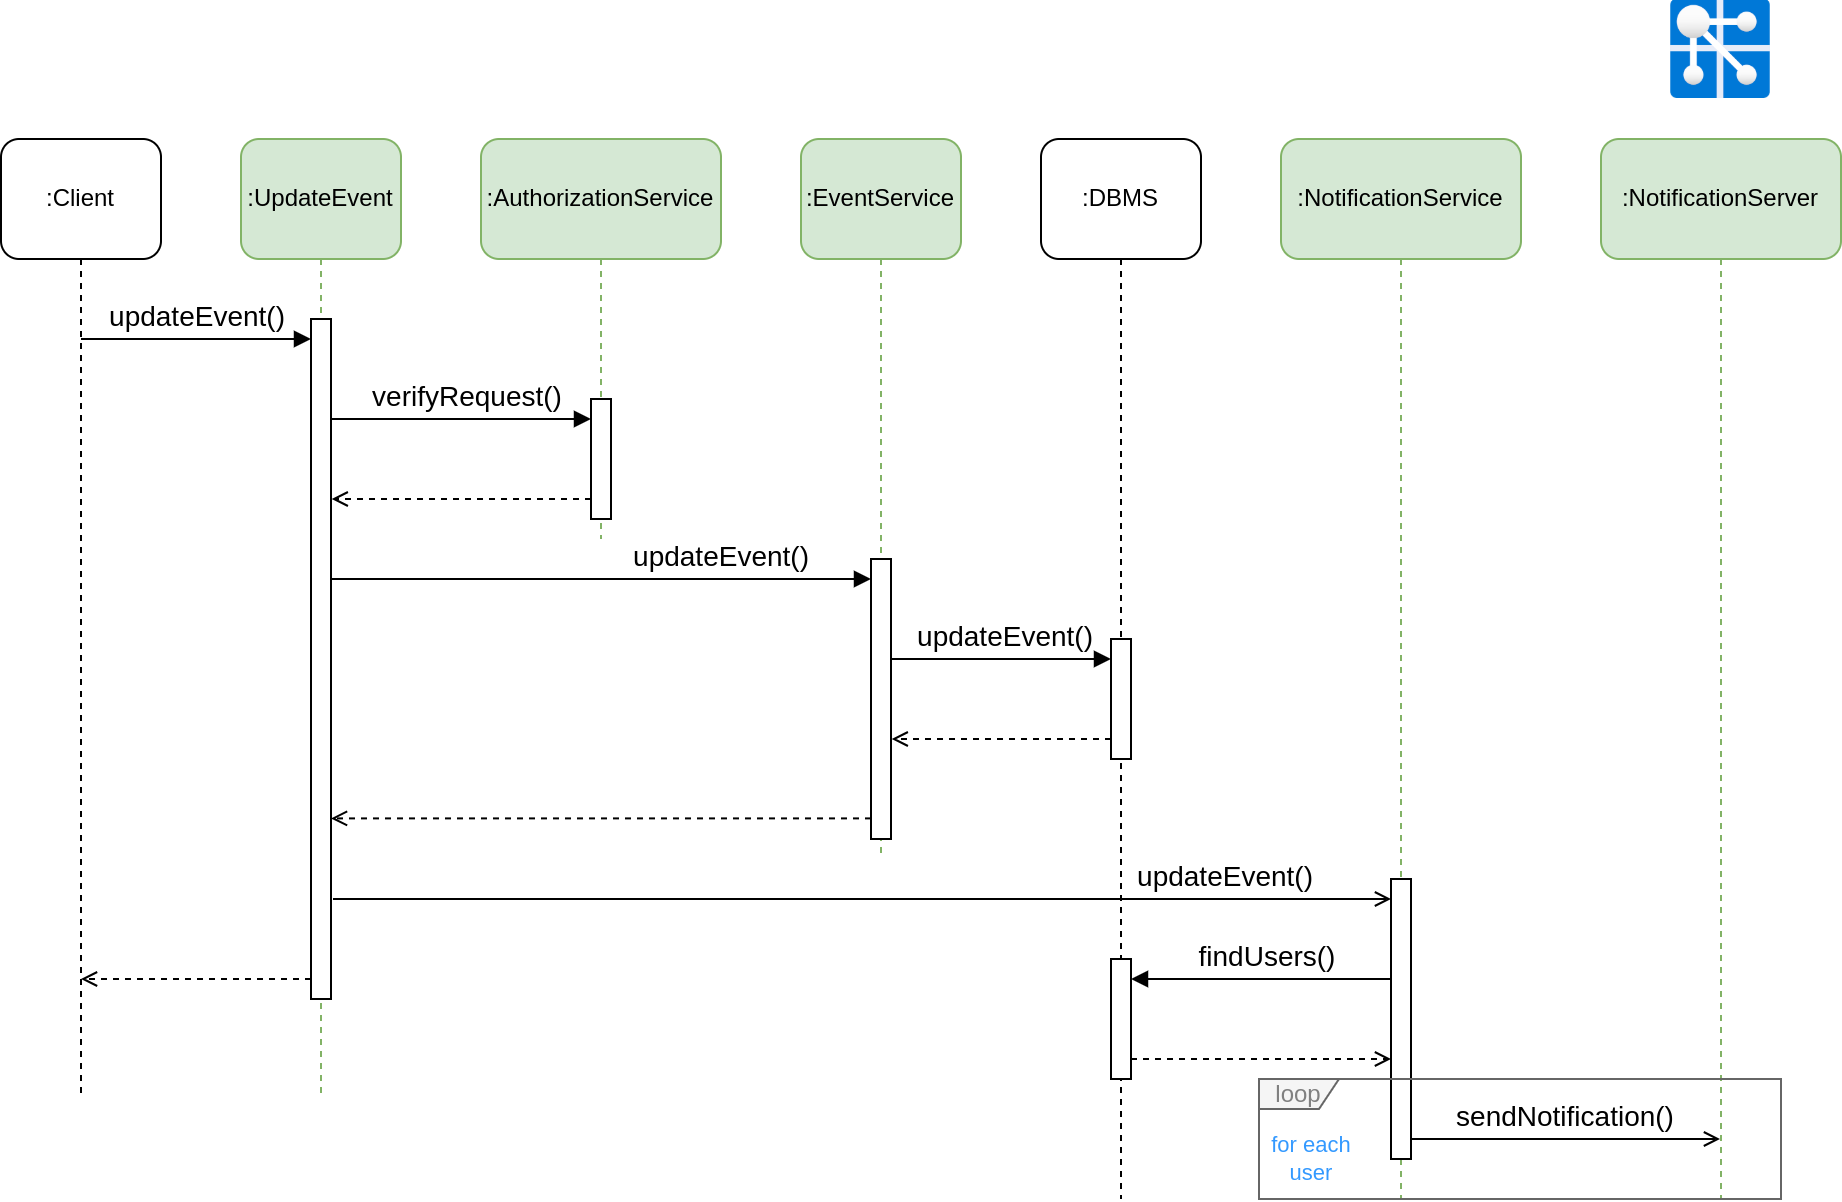
\includegraphics[width=\textwidth]{IIModificaEvento2.png}
    \caption{Interazione delle Azure Functions con AWPS}
\end{figure}	

La ricezione della notifica sul dispositivo dell’utente può comportare la richiesta al server dell’elemento modificato. 
La scelta di recuperare i dati tramite il server invece di includere i dati direttamente all’interno della notifica permette di uniformare il formato delle notifiche, 
semplificando la loro gestione e velocizzando l'invio; 
di diminuisce il volume dei dati trasmessi tramite WebSocket, 
garantendo la scalabilità delle notifiche; 
di migliorare la gestione degli errori da parte del server rendendoli più affidabili e 
di garantisce la possibilità di recuperare solo l’ultimo aggiornamento, 
riducendo il consumo totale dei dati.


\begin{figure}[h!]
    \centering
    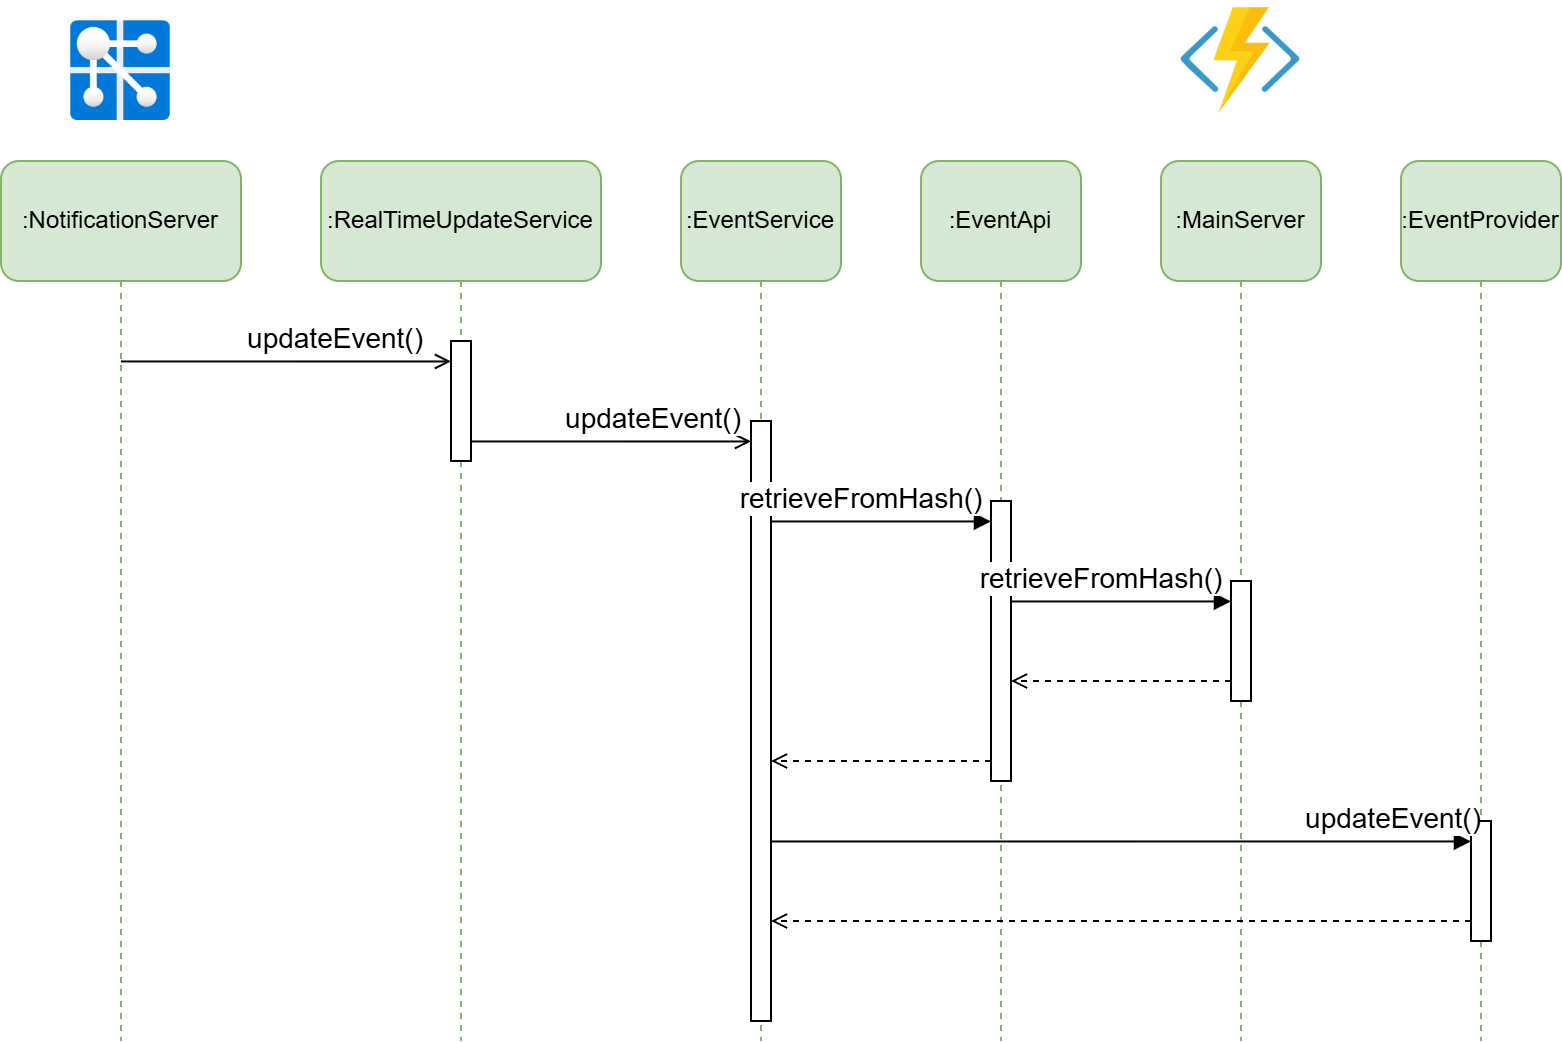
\includegraphics[width=\textwidth]{IIAggiornaEvento.png}
    \caption{Interazione tra AWPS e un client}
\end{figure}	

\clearpage